\chapter{Použité technológie, nástroje a architektonický vzor}\label{chap:technologie}
Táto kapitola analyzuje zvolené nástroje, technológie a architektonický vzor využité počas celého životného cyklu mobilnej aplikácie Office Hours – od vizuálneho návrhu a prototypovania používateľského rozhrania, cez implementáciu klientskej časti až po testovanie komunikácie s backendovými službami.

\subsubsection{Nástroje použité pri vývoji a návrhu}
\begin{itemize}
    \item \textbf{Postman:} Platforma na testovanie API, ktorá bola použitá na overovanie komunikácie s backendom, testovanie autentifikácie pomocou JWT (JSON Web Token) tokenov a kontrolu HTTP status kódov\footnote{\url{https://www.postman.com}}.

    \item \textbf{Figma:} Cloudový vektorový grafický editor využitý na tvorbu kompletných vizualizácií všetkých obrazoviek a interaktívnych prototypov používateľského rozhrania\footnote{\url{https://www.figma.com}}.

    \item \textbf{Canva:} Online grafický editor použitý na tvorbu Use Case diagramu a diagramu toku autentifikácie\footnote{\url{https://www.canva.com}}.

    \item \textbf{Coolors.co:} Webový generátor farebných schém s integrovaným Contrast Checkerom\footnote{\url{https://coolors.co}}.
\end{itemize}
\section{Použité technológie}
Nasledujúca sekcia predstavuje primárne technológie, programovacie jazyky, zvolenú architektúru a špecifické knižnice, ktoré tvoria funkčný základ mobilnej aplikácie.
\subsection{Framework Flutter a jazyk Dart}
Na vývoj mobilnej aplikácie bol použitý \textbf{Flutter} vo verzii 3.32.7 – open-source UI framework vyvinutý spoločnosťou Google~\cite{flutter}. Výber Flutteru oproti alternatívnym multiplatformovým riešeniam bol podmienený niekoľkými technickými faktormi.

Na rozdiel od React Native, ktorý pri tvorbe UI závisí od natívnych komponentov
platformy a komunikuje s nimi cez JavaScript vrstvu, čo môže spôsobovať
výkonnostnú réžiu a vizuálnu nekonzistentnosť medzi platformami (hoci nová architektúra React Native JSI/Fabric, dostupná od verzie 0.68, tieto problémy výrazne redukuje~\cite{rn_new_arch}), flutter vykresľuje všetky grafické prvky prostredníctvom vlastného enginu
Impeller (nahrádza pôvodný
engine Skia) nezávisle od operačného systému. Tento prístup zaručuje identický
vzhľad a správanie aplikácie na systémoch Android aj iOS, pričom v produkčnom zostavení Flutter kompiluje kód priamo do natívnych inštrukcií procesora~\cite{flutter_architecture}.

V porovnaní s Kotlin Multiplatform (KMP) je Flutter vhodnejší najmä pri rýchlom prototypovaní a vývoji MVP (Minimum Viable Product). KMP síce umožňuje zdieľanie biznis logiky, avšak používateľské rozhranie sa stále implementuje natívne pre každú platformu osobitne. V praxi to znamená, že Android a iOS môžu používať rovnakú logiku, ale používateľské rozhranie sa stále implementuje natívne, (napríklad pomocou Jetpack Compose na Androide a SwiftUI na iOS). Takýto prístup je výhodný pri aplikáciách, kde je prioritou natívny vzhľad a hlboká integrácia s platformou, no natívne rozhranie pre iOS si zároveň vyžaduje dodatočnú znalosť jazyka Swift/SwiftUI. Flutter naproti tomu pokrýva v jedinom projekte a jedinom jazyku (Dart) ako biznis logiku, tak aj celé používateľské rozhranie~\cite{kmp}.

Základným stavebným prvkom vo Flutteri je tzv. \textit{Widget}. Vo Flutteri je widgetom úplne všetko – od textu a tlačidla až po celkové rozloženie obrazovky (layout). Aplikácia vzniká skladaním týchto widgetov do hierarchického stromu (Widget Tree)~\cite{flutter_widget_tree}.

Aplikácie vo Flutteri sú programované v jazyku \textbf{Dart}, ktorý je rovnako vyvíjaný spoločnosťou Google. V tomto projekte bola použitá verzia Dart SDK 3.8.1. Ide o moderný, objektovo orientovaný jazyk so silnou typovou kontrolou. Jeho zásadnou výhodou pre mobilný vývoj je podpora dvoch typov kompilácie~\cite{dart2024overview}:
\begin{itemize}
    \item \textbf{JIT (Just-In-Time):} Využíva sa počas vývoja. Umožňuje funkciu Hot Reload, keď sa zmeny v kóde prejavia v bežiacej aplikácii za zlomok sekundy bez nutnosti rekompilácie.
    \item \textbf{AOT (Ahead-Of-Time):} Využíva sa pri tvorbe produkčného zostavenia (release build). Kód je skompilovaný priamo do inštrukcií procesora, čo zabezpečuje rýchly štart aplikácie a vysoký výkon na koncovom zariadení.
\end{itemize}
Jazyk Dart taktiež podporuje bezpečnosť voči nulovým hodnotám, čím sa priamo na úrovni kompilátora predchádza jednej z najčastejších chýb – chybám spôsobeným prístupom k nulovým hodnotám~\cite{dart2024nullsafety}.

\subsection{Použité knižnice (Packages)}
Projekt využíva balíčky z oficiálneho repozitára \textit{pub.dev}\footnote{\url{https://pub.dev}}. Medzi najdôležitejšie knižnice integrované do aplikácie Office Hours patria:

\begin{itemize}
    \item \textbf{http}: Slúži na tvorbu sieťových požiadaviek. Táto knižnica bola použitá na komunikáciu s dedikovaným REST API\footnote{REST API, s ktorým aplikácia komunikuje, je dostupné na:
\url{https://office-hours.fit.vutbr.cz/api/}} (odosielanie a prijímanie JSON dát pomocou metód GET, POST a DELETE).
    \item \textbf{provider}: Knižnica pre správu stavu aplikácie vo Flutteri,
    využitá na implementáciu architektúry MVVM. Konkrétny spôsob prepojenia
    ViewModelu s prezentačnou vrstvou je popísaný v sekcii~\ref{subsubsec:navrh-provider}.
    \item \textbf{get\_it}: Tento balíček slúži na centrálnu registráciu a prístup k službám, akými sú napríklad triedy \textbf{ApiService} alebo \textbf{NavigationService}, čím sa zabezpečuje čisté oddelenie zodpovedností v kóde~\cite{getit}.
    \item \textbf{shared\_preferences}: Umožňuje perzistentné ukladanie jednoduchých dátových typov (napr. používateľské preferencie, zvolená téma) do nešifrovaného lokálneho úložiska zariadenia.
    \item \textbf{flutter\_secure\_storage}: Zabezpečuje ukladanie citlivých údajov
    do šifrovaného systémového úložiska zariadenia~\cite{fluttersecurestorage}.
    V aplikácii je použitá výlučne na ukladanie JWT tokenu. Konkrétna implementácia je popísaná v sekcii~\ref{subsec:impl-secure}.
\end{itemize}

Pre vizuálne a pomocné účely boli ďalej využité nasledujúce balíčky: 
\begin{itemize}
    \item \textbf{flutter\_svg} s ikonami \textit{Heroicons}\footnote{\url{https://heroicons.com/}}: Integrácia sady ikon vo formáte SVG.
    \item \textbf{fluttertoast} a \textbf{overlay\_kit}: Zobrazovanie notifikačných správ (Toast notifications).
    \item \textbf{flutter\_spinkit}: Animované indikátory načítavania.
    \item \textbf{flutter\_native\_splash} a \textbf{flutter\_launcher\_icons}: Konfigurácia ikony aplikácie a úvodnej splash obrazovky.
    \item \textbf{intl}: Formátovanie dátumov a časov.
    \item \textbf{dropdown\_search}: Vyhľadávateľné rozbaľovacie zoznamy (autocomplete).
    \item \textbf{sticky\_headers}: Knižnica zabezpečujúca pripnutie hlavičiek sekcií pri rolovovaní zoznamom.
    \item \textbf{connectivity\_plus}: Detekcia stavu sieťového pripojenia.
    \item \textbf{jwt\_decoder}: Overenie expirácie JWT tokenu.
    \item \textbf{url\_launcher}: Otváranie externých odkazov v systémovom prehliadači.
    \item \textbf{syncfusion\_flutter\_datepicker}: Komponent kalendára s výberom dátumu.
    \item \textbf{figma\_squircle}: Tvar, ktorý je prechodom medzi štvorcom (square) a kruhom (circle).
\end{itemize}

\section{Architektonický vzor MVVM}
\label{sec:architektura-mvvm}
Bez jasne definovanej architektúry sa kód mobilnej aplikácie rýchlo stáva neudržateľným a neprehľadným. Z tohto dôvodu bol v projekte Office Hours implementovaný architektonický návrhový vzor \textbf{MVVM (Model-View-ViewModel)}.

Na pochopenie prínosu MVVM je užitočné porovnať ho so starším vzorom \textbf{MVC (Model-View-Controller)}, z ktorého vychádza. Porovnanie komunikácie medzi jednotlivými vrstvami architektúr MVC, MVP a MVVM je znázornené na obrázku~\ref{fig:mvvm}. V MVC sprostredkúva interakciu medzi dátami a rozhraním komponent Controller. Jeho zásadným problémom je \textit{smer závislosti}: Controller priamo ovláda View, drží referencie na konkrétne UI prvky a aktívne do nich tlačí zmeny (napríklad \textbf{controller.hideButton()} alebo \textbf{controller.updateLabel()}). Výsledkom je pevná väzba – akákoľvek zmena v UI si vyžaduje zásah aj do Controllera, čo kód robí krehkým a ťažko testovateľným~\cite{akhtar2021}.

Ďalším relevantným vzorom je \textbf{MVP (Model-View-Presenter)}, ktorý priamo predchádza MVVM a rieši niektoré nedostatky MVC. Presenter úplne oddeľuje vrstvu Model od vrstvy View, View a Presenter komunikujú prostredníctvom explicitného rozhrania (interface), čo výrazne uľahčuje testovanie. Nevýhodou MVP je však to, že s rastom projektu sa Presenter môže stať rozsiahlou triedou s množstvom metód, čo komplikuje jeho pochopenie a údržbu~\cite{akhtar2021}.

Pri MVVM je ViewModel úplne nezávislý od View~\cite{akhtar2021}. ViewModel namiesto priamych volaní na View vystavuje pozorovateľný stav – napríklad pomocou \textbf{StateFlow} v Kotline alebo \textbf{ObservableObject} v SwiftUI – a View sa naň prihlási ako pozorovateľ.

Tento vzor striktne rozdeľuje aplikačný kód do troch hlavných vrstiev:
\begin{itemize}
    \item \textbf{Model (Dátová vrstva):} Obsahuje definície dátových štruktúr a služby zodpovedné za komunikáciu s externým API. Táto vrstva nemá žiadnu vedomosť o používateľskom rozhraní.
    \item \textbf{View (Prezentačná vrstva):} Zodpovedá výlučne za vizualizáciu dát. Vo Flutteri ide o sadu widgetov, ktoré zobrazujú stav z ViewModelu a predávajú mu informácie o používateľských interakciách, ako sú kliknutia alebo gestá.
    \item \textbf{ViewModel (Logická medzivrstva):} Slúži ako most medzi Modelom a View. Udržiava aktuálny stav obrazovky, spracováva vstupy a transformuje dáta získané z Modelu do formátu zobraziteľného v UI.
\end{itemize}

\begin{figure}[t]
    \centering
    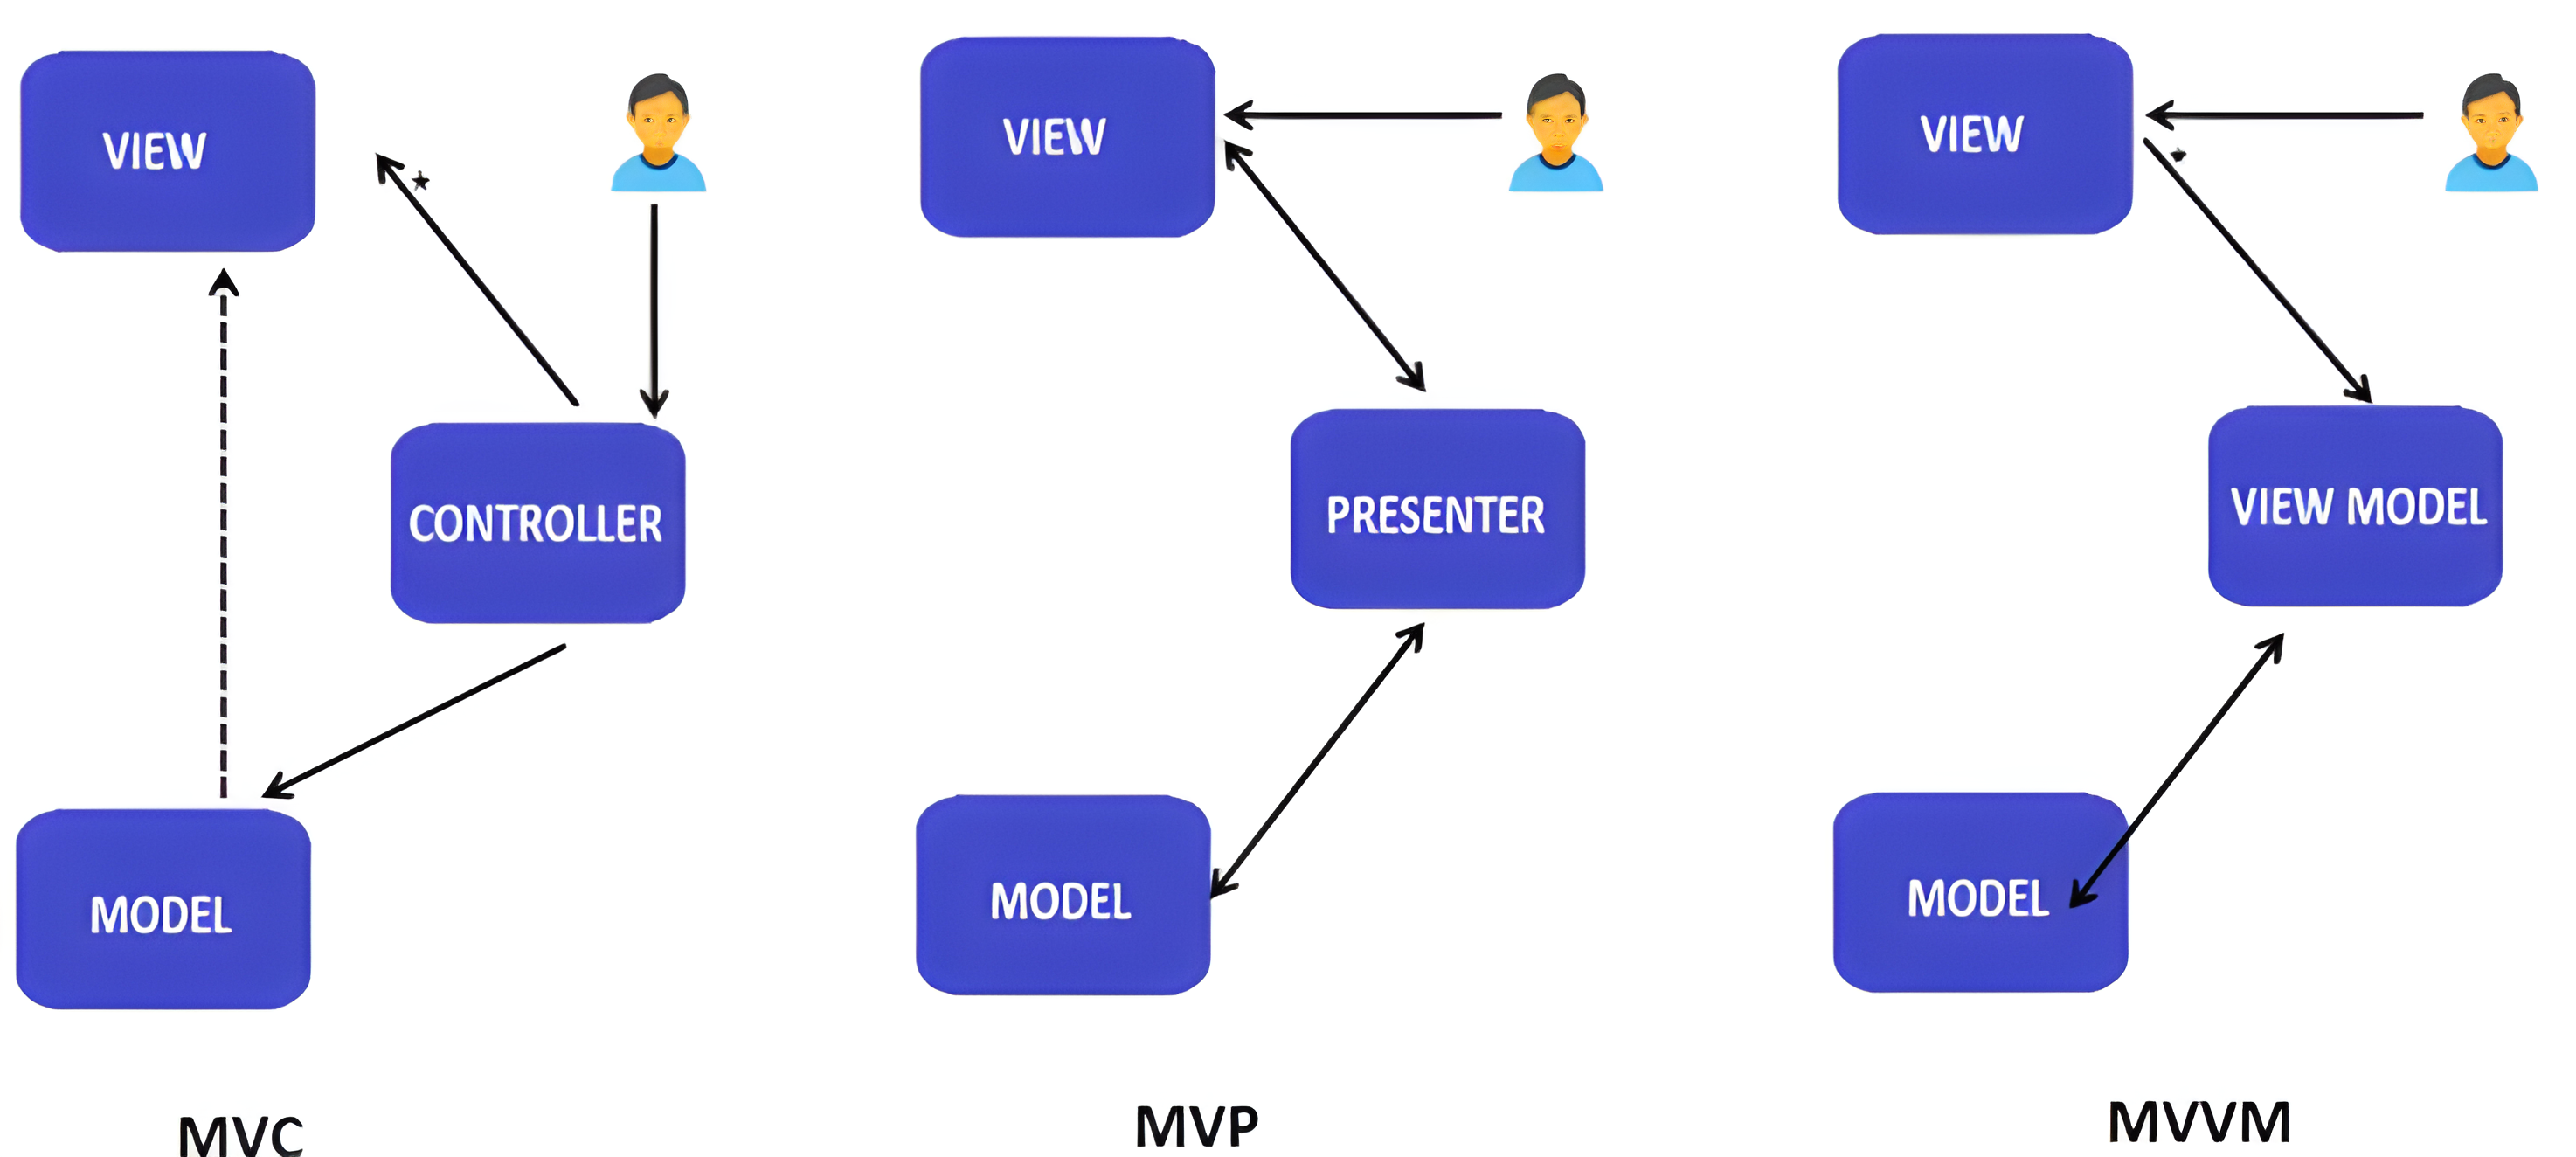
\includegraphics[width=1\textwidth]{obrazky-figures/tech-mvvm-comparasion.png}
    \caption{Porovnanie architektonických vzorov MVC, MVP a MVVM – znázornenie komunikácie medzi používateľom, View, Modelom a riadiacimi komponentmi. Zdroj: \cite{sinhal2016mvc}}
    \label{fig:mvvm}
\end{figure}

\subsection{Reaktívne prepojenie View a ViewModelu}
\label{subsubsec:navrh-provider}
V projekte Office Hours je reaktívne prepojenie medzi View a ViewModelom zabezpečené prostredníctvom balíčka \textbf{provider}~\cite{provider} v kombinácii s triedou \textbf{ChangeNotifier}. Toto riešenie je postavené na návrhovom vzore \textbf{Pozorovateľ} (Observer pattern).

Princíp fungovania je nasledovný: keď ViewModel vykoná asynchrónnu operáciu (napríklad odošle požiadavku na server), zmení svoj lokálny stav a zavolá metódu \textbf{notifyListeners()}. Toto volanie upozorní framework Flutter, aby prekreslil \emph{výlučne} tú časť používateľského rozhrania, ktorá počúva na zmeny daného ViewModelu. Vďaka tomuto selektívnemu prístupu nedochádza k zbytočnému prekresľovaniu celej obrazovky, čo šetrí systémové prostriedky a prispieva k plynulosti aplikácie.